\newpage
\section{Implémentation et Algorithmes}

\subsection{Tokenization}

La première étape du pipeline consiste à découper le texte en tokens. Nous avons appliqué :

\begin{algorithm}[H]
\caption{Tokenization}
\begin{algorithmic}[1]
\State \textbf{Entrée} : Texte brut $T$
\State \textbf{Sortie} : Liste de tokens $L$
\State Convertir $T$ en minuscules
\State Supprimer la ponctuation
\State Découper $T$ en mots (tokens)
\State Supprimer les stopwords de $T$
\State Appliquer la lemmatisation sur les tokens
\State \textbf{Retourner} $L$
\end{algorithmic}
\end{algorithm}
\textbf{Complexité :}  
La complexité de la tokenisation dépend du type d’approche utilisée :
\begin{itemize}
    \item Pour une tokenization basée sur des expressions régulières : 
    \begin{equation}
    O(n)
    \end{equation}
    où \( n \) est la longueur du texte.
    \item Pour une tokenization basée sur un dictionnaire avec recherche binaire :
    \begin{equation}
    O(n \log k)
    \end{equation}
    où \( k \) est la taille du dictionnaire.
\end{itemize}

\subsection{Extraction des caractéristiques} Cette étape transforme les tokens générés précédemment en représentations numériques exploitables par les algorithmes d'apprentissage automatique.

Nous avons utilisé deux méthodes :
\begin{itemize}
    \item \textbf{CountVectorizer} : Nombre d’occurrences de chaque mot
    \item \textbf{TF-IDF} : Importance relative des mots
\end{itemize}
Pour cela on distingue 2 parties principales:
\begin{itemize}
    \item[•] {Indexation} : Associe un index unique à chaque mot du vocabulaire.
    \item[•] {Représentation} : Génère une matrice où :
    \begin{itemize}
        \item[] Chaque ligne représente un document.
        \item[] Chaque colonne correspond à un mot du vocabulaire.
    \end{itemize}
\end{itemize}
\subsubsection{CountVectorizer}
CountVectorizer transforme un texte en une matrice de fréquences des mots.
\begin{algorithm}[H]
\caption{CountVectorizer}
\begin{algorithmic}[1]
\State \textbf{Entrée} : Liste de documents de test $D = \{d_1, d_2, \dots, d_N\}$
\State \textbf{Sortie} : Matrice de fréquence des termes $M$
\For{\textbf{chaque document} $d_i$}
    \For{\textbf{chaque mot} $w_j$ dans $d_i$}
        \State $M[i,j] \gets \text{nombre de fois que } w_j \text{ apparait dans } d_i$
    \EndFor
\EndFor
\State \textbf{Retourner} la matrice $M$
\end{algorithmic}
\end{algorithm}
\textbf{Complexité :}  
La transformation d’un corpus contenant \( n \) documents et \( m \) mots uniques dans le vocabulaire est :
\begin{equation}
O(n \cdot m)
\end{equation}
où :
\begin{itemize}
    \item \( n \) : nombre de documents.
    \item \( m \) : nombre total de mots uniques.
\end{itemize}

\subsubsection{TF-IDF}
Cette d’extraction de caractéristiques textuelles Pondère les mots en fonction de :
    \begin{itemize}
        \item[-] Leur fréquence dans un document.
        \item[-] Leur rareté dans l’ensemble du corpus.
    \end{itemize}
L’équation de TF-IDF est :

\[
\text{TF-IDF}(t,d) = \text{TF}(t,d) \times \log \frac{N}{\text{DF}(t)}
\]
où :
\begin{itemize}
    \item \( TF(t, d) \) : fréquence du terme \( t \) dans le document \( d \).
    \item \( f_t \) : nombre d’occurrences du terme \( t \) dans \( d \).
    \item \( N \) : nombre total de mots dans \( d \).
    \item \( IDF(t) \) : inverse de la fréquence du document.
    \item \( N_d \) : nombre total de documents.
    \item \( N_t \) : nombre de documents contenant le terme \( t \).
\end{itemize}
\begin{algorithm}[H]
\caption{Calcul de TF-IDF}
\begin{algorithmic}[1]
\State \textbf{Entrée} : Liste de documents $D = \{d_1, d_2, \dots, d_N\}$
\State \textbf{Sortie} : Matrice TF-IDF $M$
\For{\textbf{chaque document} $d_i$}
    \For{\textbf{chaque terme} $t_j$ dans $d_i$}
        \State $\text{TF}(t_j, d_i) \gets \frac{\text{nombre de fois que } t_j \text{ apparait dans } d_i}{\text{total des mots dans } d_i}$
        \State $\text{DF}(t_j) \gets \text{nombre de documents contenant } t_j$
        \State $\text{IDF}(t_j) \gets \log \left( \frac{N}{\text{DF}(t_j)} \right)$
        \State $M[i,j] \gets \text{TF}(t_j, d_i) \times \text{IDF}(t_j)$
    \EndFor
\EndFor
\State \textbf{Retourner} la matrice TF-IDF $M$
\end{algorithmic}
\end{algorithm}
\textbf{Complexité :}  
Le calcul du TF-IDF a une complexité de :
\begin{equation}
O(n \cdot m)
\end{equation}
où :
\begin{itemize}
    \item \( n \) : nombre de documents.
    \item \( m \) : nombre de mots uniques dans le corpus.
\end{itemize}

\subsection{Modéles de classification}
A ce niveau les matrices de caractéristiques sont Utilisées pour entraîner le classificateur et prédire si un document est un "plagiat" ou "non plagiat".

\subsubsection{Naïve Bayes}
\begin{equation}
P(y|X) = \frac{P(X|y) P(y)}{P(X)}
\end{equation}
où :
\begin{itemize}
    \item[-] \( P(y|X) \) : probabilité a posteriori de la classe \( y \) sachant les caractéristiques \( X \).
    \item[-] \( P(X|y) \) : probabilité d’observer \( X \) sachant que l’étiquette est \( y \).
    \item[-] \( P(y) \) : probabilité a priori de la classe \( y \).
    \item[-] \( P(X) \) : probabilité totale d’observer \( X \).
\end{itemize}
\begin{algorithm}[H]
\caption{Naïve Bayes pour classification}
\begin{algorithmic}[1]
\State \textbf{Entrée} : Ensemble de données d'entraînement $\{(x_i, y_i)\}$, où $x_i$ est un vecteur de caractéristiques et $y_i$ est la classe
\State \textbf{Sortie} : Modèle de classification
\For{\textbf{chaque} classe $y$}
    \State Calculer la probabilité a priori $\hat{P}(y) = \frac{\text{nombre de } y \text{ dans les données d'entraînement}}{N}$
\EndFor
\For{\textbf{chaque} caractéristique $x_j$}
    \State Estimer la probabilité conditionnelle $\hat{P}(x_j | y)$ en utilisant les données d'entraînement
\EndFor
\State \textbf{Retourner} le modèle avec $\hat{P}(y)$ et $\hat{P}(x_j | y)$
\end{algorithmic}
\end{algorithm}
\textbf{Complexité :}  
L'entraînement de Naïve Bayes consiste à calculer les probabilités conditionnelles pour chaque attribut et chaque classe.  
\begin{equation}
O(n \cdot m)
\end{equation}
où :
\begin{itemize}
    \item \( n \) : nombre d'échantillons dans l'ensemble d'entraînement.
    \item \( m \) : nombre de caractéristiques (features).
\end{itemize}
La classification d’un nouvel échantillon se fait en :
\begin{equation}
O(m \cdot k)
\end{equation}
où \( k \) est le nombre de classes.

\subsubsection{Logistic Regression}
\begin{equation}
P(y=1|X) = \frac{1}{1 + e^{-(wX + b)}}
\end{equation}
où :
\begin{itemize}
    \item[-] \( P(y=1|X) \) : probabilité que \( X \) appartienne à la classe \( y=1 \).
    \item[-] \( w \) : vecteur des poids associés aux caractéristiques.
    \item[-] \( X \) : vecteur des caractéristiques de l'instance.
    \item[-] \( b \) : biais du modèle.
    \item[-] \( e \) : base du logarithme naturel (\(\approx 2.718\)).
\end{itemize}
\begin{figure}[H]
            \centering
            \begin{subfigure}[b]{0.4\textwidth}
                \centering
                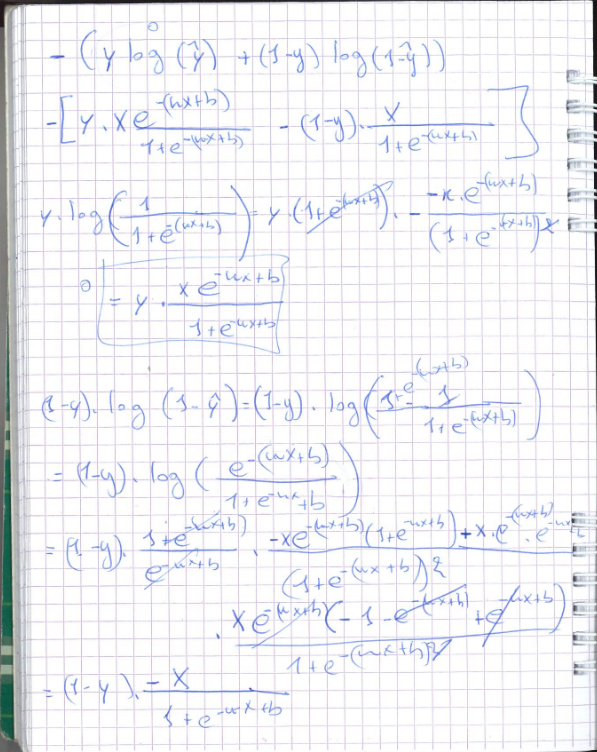
\includegraphics[width=\textwidth]{LR_db1.png}
                \caption{Original Image}
                \label{fig:original}
            \end{subfigure}
            \begin{subfigure}[b]{0.4\textwidth}
                \centering
                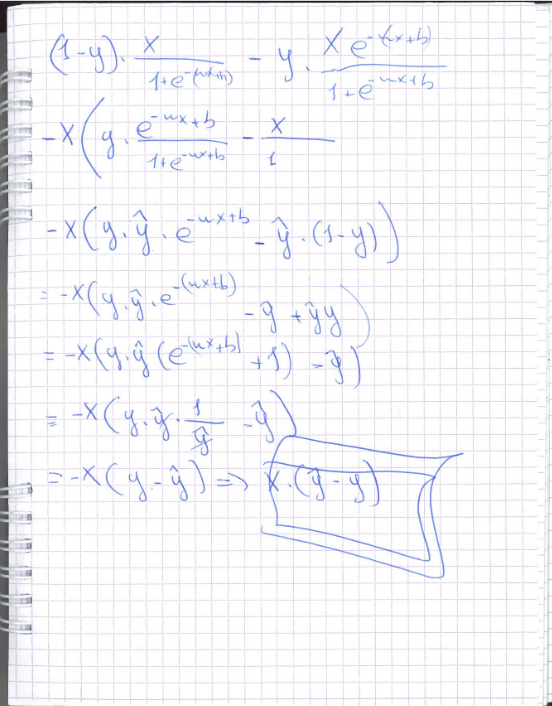
\includegraphics[width=\textwidth]{LR_dw2.png}
                \caption{After Histogram Normalization}
                \label{fig:original}
            \end{subfigure}
            \caption{ Calcule de Dw }
            \label{fig:cam_man_hn}
\end{figure}
\begin{figure}[H]
            \centering
            \begin{subfigure}[b]{0.4\textwidth}
                \centering
                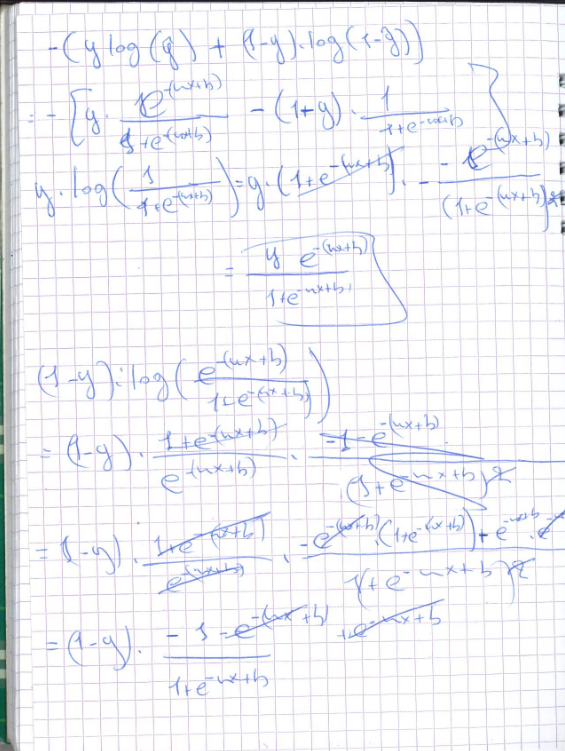
\includegraphics[width=\textwidth]{LR_dw1.png}
                \caption{Original Image}
                \label{fig:original}
            \end{subfigure}
            \begin{subfigure}[b]{0.4\textwidth}
                \centering
                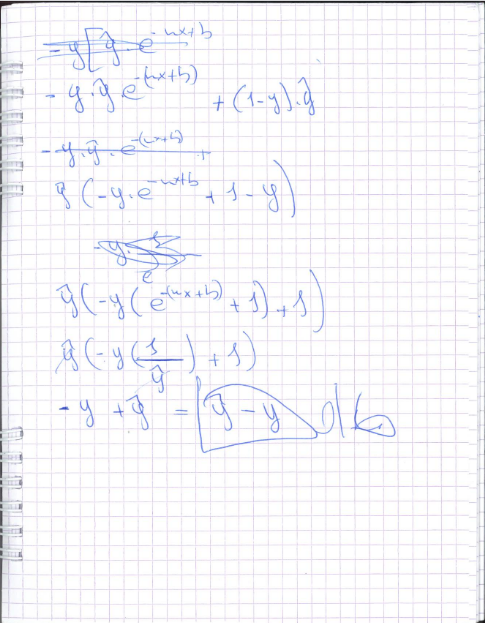
\includegraphics[width=\textwidth]{LR_db2.png}
                \caption{After Histogram Normalization}
                \label{fig:original}
            \end{subfigure}
            \caption{ Calcule de Db }
            \label{fig:cam_man_hn}
\end{figure}
\begin{algorithm}[H]
\caption{Régression Logistique pour classification}
\begin{algorithmic}[1]
\State \textbf{Entrée} : Ensemble de données d'entraînement $\{(x_i, y_i)\}$, où $x_i$ est un vecteur de caractéristiques et $y_i$ est la classe
\State Initialiser les poids $w$ et le biais $b$
\For{\textbf{chaque} échantillon $(x_i, y_i)$}
    \State Calculer la probabilité $\hat{y_i} = \sigma(w \cdot x_i + b)$, où $\sigma(z) = \frac{1}{1 + e^{-z}}$
    \State Calculer l'erreur $L = y_i \log(\hat{y_i}) + (1 - y_i) \log(1 - \hat{y_i})$
    \State Mettre à jour les poids $w$ et $b$ avec la descente de gradient :
    \State $w = w - \eta \frac{\partial L}{\partial w}$
    \State $b = b - \eta \frac{\partial L}{\partial b}$
\EndFor
\State \textbf{Retourner} $w, b$
\end{algorithmic}
\end{algorithm}
\textbf{Complexité :}  
L'entraînement est effectué via la descente de gradient, qui prend :
\begin{equation}
O(i \cdot n \cdot m)
\end{equation}
où :
\begin{itemize}
    \item \( i \) : nombre d'itérations.
    \item \( n \) : nombre d'échantillons.
    \item \( m \) : nombre de caractéristiques.
\end{itemize}
La classification d’un nouvel échantillon se fait en :
\begin{equation}
O(m)
\end{equation}

\subsubsection{Perceptron}
\begin{equation}
y = \text{sign}(wX + b)
\end{equation}
où :
\begin{itemize}
    \item \( y \) : classe prédite (\(+1\) ou \(-1\)).
    \item \( \text{sign}(z) \) : fonction qui retourne \( +1 \) si \( z \) est positif, sinon \( -1 \).
    \item \( w \) : vecteur des poids.
    \item \( X \) : vecteur des caractéristiques.
    \item \( b \) : biais.
\end{itemize}

\begin{figure}[H]
    \centering
    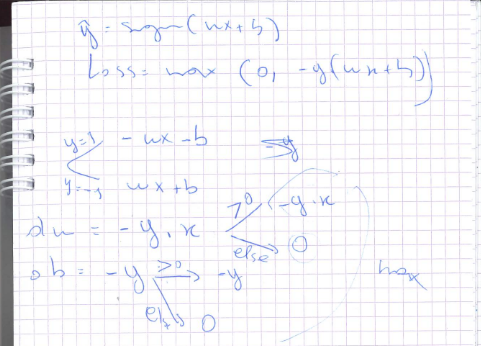
\includegraphics[width=0.5\linewidth]{perceptron.png}
    \caption{Calcule de Decent Gradient}
    \label{fig:mon_image}
\end{figure}

\begin{algorithm}[H]
\caption{Perceptron pour classification binaire}
\begin{algorithmic}[1]
\State \textbf{Initialisation} : poids $w$, biais $b$, taux d'apprentissage $\eta$
\For{\textbf{chaque} échantillon $(x_i, y_i)$}
    \State $\hat{y} = \text{sign}(w \cdot x_i + b)$
    \If{$\hat{y} \neq y_i$}
        \State $w = w + \eta (y_i x_i)$
        \State $b = b + \eta y_i$
    \EndIf
\EndFor
\State \textbf{Retourner} $w, b$
\end{algorithmic}
\end{algorithm}

\textbf{Complexité :}  
L'algorithme du perceptron apprend en ajustant les poids en fonction des erreurs. Sa complexité d'entraînement est :
\begin{equation}
O(i \cdot n \cdot m)
\end{equation}
et la classification d’un nouvel échantillon se fait en :
\begin{equation}
O(m)
\end{equation}

\subsubsection{Decision Tree}
\paragraph{Indice de Gini}
\begin{equation}
Gini = 1 - \sum p_i^2
\end{equation}
où :
\begin{itemize}
    \item[-] \( Gini \) : mesure d'impureté du nœud.
    \item[-] \( p_i \) : proportion d’éléments appartenant à la classe \( i \) dans le nœud.
\end{itemize}

\paragraph{Entropie}
\begin{equation}
Entropy = -\sum p_i \log_2 p_i
\end{equation}
où :
\begin{itemize}
    \item[-] \( Entropy \) : mesure d’incertitude dans la répartition des classes.
    \item[-] \( p_i \) : proportion d’éléments de la classe \( i \) dans le nœud.
    \item[-] \( \log_2 \) : logarithme en base 2.
\end{itemize}
\begin{algorithm}[H]
\caption{Arbre de Décision pour classification}
\begin{algorithmic}[1]
\State \textbf{Entrée} : Ensemble de données d'entraînement $\{(x_i, y_i)\}$, où $x_i$ est un vecteur de caractéristiques et $y_i$ est la classe
\State \textbf{Sortie} : Arbre de décision
\State Construire l'arbre récursivement :
    \For{\textbf{chaque} noeud de l'arbre}
        \State Calculer l'impureté (par exemple, entropie ou Gini) pour chaque caractéristique
        \State Choisir la caractéristique qui minimise l'impureté (meilleure séparation)
        \State Diviser l'ensemble de données en fonction de la caractéristique choisie
        \State Si le noeud est pur (impureté = 0) ou si un critère d'arrêt est atteint, arrêter
    \EndFor
\State \textbf{Retourner} l'arbre construit
\end{algorithmic}
\end{algorithm}
\textbf{Complexité :}  
L'entraînement d'un arbre de décision nécessite la recherche du meilleur attribut pour la division des données à chaque nœud. Cette opération a une complexité :
\begin{equation}
O(n \cdot m \log n)
\end{equation}
La classification d’un nouvel échantillon prend :
\begin{equation}
O(d)
\end{equation}
où \( d \) est la profondeur de l’arbre.



\subsubsection{Bagging (Bootstrap Aggregating)}

Bagging est une méthode d'ensemble qui vise à réduire la variance des modèles d'apprentissage supervisé. Il repose sur la création de plusieurs sous-échantillons des données d'entraînement en effectuant un \textbf{bootstrap sampling} (tirage avec remise). Chaque modèle est entraîné indépendamment sur un sous-échantillon et leurs prédictions sont ensuite combinées pour obtenir un modèle plus robuste. Le RandomForest en est une extension (un Bagging sur des arbres de décision).

\paragraph{Algorithme de Bagging}

\begin{algorithm}[H]
\caption{Algorithme de Bagging}
\begin{algorithmic}[1]
\State \textbf{Entrée} : Ensemble d'entraînement \( D \) de taille \( N \), Nombre de modèles \( M \), Modèle de base \( h \)
\For{$t = 1$ \textbf{to} $M$}
    \State Générer un échantillon \( D_t \) en tirant \( N \) instances de \( D \) avec remise.
    \State Entraîner un modèle \( h_t \) sur \( D_t \)
\EndFor
\State \textbf{Prédiction} :
\If{Classification}
    \State Retourner la majorité des prédictions des \( M \) modèles : \( \text{majorité}(h_1(x), h_2(x), ..., h_M(x)) \)
\Else
    \State Retourner la moyenne des prédictions des \( M \) modèles : \( \frac{1}{M} \sum_{t=1}^{M} h_t(x) \)
\EndIf
\end{algorithmic}
\end{algorithm}


\subsubsection{AdaBoost (Adaptive Boosting)}

AdaBoost est une technique de \textbf{boosting} qui combine plusieurs classificateurs faibles pour créer un modèle robuste. Contrairement au bagging, AdaBoost entraîne les modèles \textbf{séquentiellement} en pondérant les erreurs : les exemples mal classés reçoivent un poids plus important à chaque itération pour forcer le modèle suivant à mieux les apprendre.

\paragraph{Algorithme d'AdaBoost}

\begin{algorithm}[H]
\caption{Algorithme d'AdaBoost}
\begin{algorithmic}[1]
\State \textbf{Entrée} : Ensemble d'entraînement \( D = \{(x_1, y_1), ..., (x_N, y_N)\} \), Nombre de modèles \( M \), Modèle faible \( h \), Poids initialisés uniformément : \( w_i = \frac{1}{N} \)
\For{$t = 1$ \textbf{to} $M$}
    \State Entraîner un classificateur \( h_t \) sur les données pondérées \( (D, w) \)
    \State Calculer l'erreur pondérée \( e_t = \sum_{i=1}^{N} w_i \cdot \mathbb{1}(h_t(x_i) \neq y_i) \)
    \State Calculer le poids du modèle \( \alpha_t = \frac{1}{2} \ln \left(\frac{1 - e_t}{e_t}\right) \)
    \State Mettre à jour les poids des échantillons :
    \[
    w_i \leftarrow w_i \cdot e^{-\alpha_t y_i h_t(x_i)}
    \]
    \State Normaliser les poids \( w_i \) pour que \( \sum w_i = 1 \)
\EndFor
\State \textbf{Prédiction} : 
\State Prédire la classe pour un nouvel exemple \( x \) : 

H(x) = \text{sign} \left( \sum_{t=1}^{M} \alpha_t h_t(x) \right)
\end{algorithmic}
\end{algorithm}
